\chapter{Introduction}\label{introduction}

\section{Motivation for Dakota Development}\label{introduction:motivation}

Computational models are commonly used in engineering design and
scientific discovery activities for simulating complex physical
systems in disciplines such as fluid mechanics, structural dynamics,
heat transfer, nonlinear structural mechanics, shock physics, and many
others. These simulators can be an enormous aid to engineers who want
to develop an understanding and/or predictive capability for complex
behaviors typically observed in the corresponding physical
systems. Simulators often serve as virtual prototypes, where a set of
predefined system parameters, such as size or location dimensions and
material properties, are adjusted to improve the performance of a
system, as defined by one or more system performance objectives. Such
optimization or tuning of the virtual prototype requires executing the
simulator, evaluating performance objective(s), and adjusting the
system parameters in an iterative, automated, and directed way. System
performance objectives can be formulated, for example, to minimize
weight, cost, or defects; to limit a critical temperature, stress, or
vibration response; or to maximize performance, reliability,
throughput, agility, or design robustness.  In addition, one would
often like to design computer experiments, run parameter studies, or
perform uncertainty quantification. These approaches reveal how system
performance changes as a design or uncertain input variable changes.
Sampling strategies are often used in uncertainty quantification to
calculate a distribution on system performance measures, and to
understand which uncertain inputs contribute most to the variance of
the outputs.

A primary goal for Dakota (Design Analysis Kit for Optimization and
Terascale Applications) development is to provide engineers and other
disciplinary scientists with a systematic and rapid means to obtain
improved or optimal designs or understand sensitivity or uncertainty
using simulation-based models. These capabilities generally lead to
improved designs and system performance in earlier design stages,
alleviating dependence on physical prototypes and testing, shortening
design cycles, and reducing product development costs. In addition to
providing this practical environment for answering system performance
questions, the Dakota toolkit provides an extensible platform for the
research and rapid prototyping of customized methods and
strategies~\cite{Eld98b}.

\section{Capabilities of Dakota}\label{introduction:capabilities}

The Dakota toolkit provides a flexible, extensible interface between
your simulation code and a variety of iterative methods and
strategies. While Dakota was originally conceived as an easy-to-use
interface between simulation codes and optimization algorithms, recent
versions have been expanded to interface with other types of iterative
analysis methods such as uncertainty quantification with
nondeterministic propagation methods, parameter estimation with
nonlinear least squares solution methods, and sensitivity/variance
analysis with general-purpose design of experiments and parameter
study capabilities. These capabilities may be used on their own or as
building blocks within more sophisticated strategies such as hybrid
optimization, surrogate-based optimization, or optimization under
uncertainty.

Thus, one of the primary advantages that Dakota has to offer is that
access to a broad range of iterative capabilities can be obtained
through a single, relatively simple interface between Dakota and your
simulator. Should you want to try a different type of iterative method
or strategy with your simulator, it is only necessary to change a few
commands in the Dakota input and start a new analysis. The need to
learn a completely different style of command syntax and the need to
construct a new interface each time you want to use a new algorithm
are eliminated.

\section{How Does Dakota Work?}\label{introduction:how}

Figure~\ref{introduction:bbinterface} depicts a typical
loosely-coupled, or ``black-box,'' relationship between Dakota and the
simulation code(s).  Such loose coupling is the simplest and most
common interfacing approach Dakota users employ. Data is exchanged
between Dakota and the simulation code by reading and writing short
data files, thus using Dakota does not require the source code of the
simulation software. Dakota is executed using commands that the user
supplies in an input file (not shown in
Figure~\ref{introduction:bbinterface}) which specify the type of
analysis to be performed (e.g., parameter study, optimization,
uncertainty quantification, etc.), along with the file names
associated with the user's simulation code. During its operation,
Dakota automatically executes the user's simulation code by creating a
separate process external to Dakota.

\begin{figure}
  \centering
  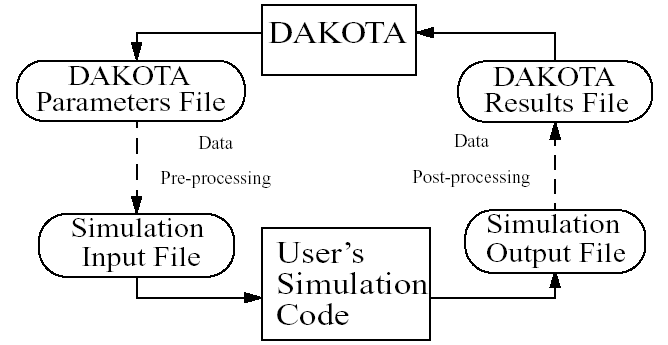
\includegraphics[scale=0.60]{images/dakota_flowchart}
  \caption{The loosely-coupled or ``black-box'' interface between
    Dakota and a user-supplied simulation code.}
  \label{introduction:bbinterface}
\end{figure}

The solid lines in Figure~\ref{introduction:bbinterface} denote file
input/output (I/O) operations that are part of Dakota or the user's
simulation code. The dotted lines indicate the passing/conversion of
information that must be implemented by the user. As Dakota runs, it
writes out a parameters file containing the current variable values.
Dakota then starts the user's simulation code (or, often, a short
driver script wrapping it), and when the simulation completes, reads
the response data from a results file. This process is repeated until
all of the simulation code runs required by the iterative study are
complete.

In some cases it is advantageous to have a close coupling between
Dakota and the simulation code. This close coupling is an advanced
feature of Dakota and is accomplished through either a direct
interface or a SAND (simultaneous analysis and design) interface. For
the direct interface, the user's simulation code is modified to behave
as a function or subroutine under Dakota. This interface can be
considered to be ``semi-intrusive'' in that it requires relatively
minor modifications to the simulation code. Its major advantage is the
elimination of the overhead resulting from file I/O and process
creation. It can also be a useful tool for parallel processing, by
encapsulating everything within a single executable. A SAND interface
approach is ``fully intrusive'' in that it requires further
modifications to the simulation code so that an optimizer has access
to the internal residual vector and Jacobian matrices computed by the
simulation code. In a SAND approach, both the optimization method and
a nonlinear simulation code are converged simultaneously. While this
approach can greatly reduce the computational expense of optimization,
considerable software development effort must be expended to achieve
this intrusive coupling between SAND optimization methods and the
simulation code.  SAND may be supported in future Dakota releases.

\section{Background and Mathematical Formulations}\label{introduction:background}

This section provides a basic introduction to the mathematical
formulation of optimization, nonlinear least squares, sensitivity
analysis, design of experiments, and uncertainty quantification
problems. The primary goal of this section is to introduce terms
relating to these topics, and is not intended to be a description of
theory or numerical algorithms. There are numerous sources of
information on these topics
(\cite{Aro89},~\cite{Gil81},~\cite{Haf92},~\cite{Hal00},~\cite{Noc99},~\cite{Van84}) and
the interested reader is advised to consult one or more of these
texts.

\subsection{Optimization}\label{introduction:background:optimization}

A general optimization problem is formulated as follows:

\begin{eqnarray}
  \hbox{minimize:} & & f(\mathbf{x})\nonumber\\
  & & \mathbf{x} \in \Re^{n}\nonumber\\
  \hbox{subject to:} & &
  \mathbf{g}_{L} \leq \mathbf{g(x)} \leq \mathbf{g}_U\nonumber\\
  & & \mathbf{h(x)}=\mathbf{h}_{t}\label{introduction:equation01}\\
  & & \mathbf{a}_{L} \leq \mathbf{A}_i\mathbf{x} \leq
  \mathbf{a}_U\nonumber\\
  & & \mathbf{A}_{e}\mathbf{x}=\mathbf{a}_{t}\nonumber\\
  & & \mathbf{x}_{L} \leq \mathbf{x} \leq \mathbf{x}_U\nonumber
\end{eqnarray}

where vector and matrix terms are marked in bold typeface. In this
formulation, $\mathbf{x}=[x_{1},x_{2},\ldots,x_{n}]$ is an
n-dimensional vector of real-valued \emph{design variables} or
\emph{design parameters}. The n-dimensional vectors, $\mathbf{x}_{L}$
and $\mathbf{x}_U$, are the lower and upper bounds, respectively, on
the design parameters. These bounds define the allowable values for
the elements of $\mathbf{x}$, and the set of all allowable values is
termed the \emph{design space} or the \emph{parameter space}. A
\emph{design point} or a \emph{sample point} is a particular set of 
values within the parameter space.

The optimization goal is to minimize the \emph{objective function},
$f(\mathbf{x})$, while satisfying the constraints.  Constraints can be
categorized as either linear or nonlinear and as either inequality or
equality. The \emph{nonlinear inequality constraints},
$\mathbf{g(x)}$, are ``2-sided,'' in that they have both lower and
upper bounds, $\mathbf{g}_L$ and $\mathbf{g}_U$, respectively. The
\emph{nonlinear equality constraints}, $\mathbf{h(x)}$, have target
values specified by $\mathbf{h}_{t}$.  The linear inequality
constraints create a linear system $\mathbf{A}_i\mathbf{x}$, where
$\mathbf{A}_i$ is the coefficient matrix for the linear system.  These
constraints are also 2-sided as they have lower and upper bounds,
$\mathbf{a}_L$ and $\mathbf{a}_U$, respectively. The linear equality
constraints create a linear system $\mathbf{A}_e\mathbf{x}$, where
$\mathbf{A}_e$ is the coefficient matrix for the linear system and
$\mathbf{a}_{t}$ are the target values.  The constraints partition the
parameter space into feasible and infeasible regions. A design point
is said to be \emph{feasible} if and only if it satisfies all of the
constraints. Correspondingly, a design point is said to be
\emph{infeasible} if it violates one or more of the constraints.

Many different methods exist to solve the optimization problem given
by Equation~\ref{introduction:equation01}, all of which iterate on
$\mathbf{x}$ in some manner.  That is, an initial value for each
parameter in $\mathbf{x}$ is chosen, the \emph{response quantities},
$f(\mathbf{x})$, $\mathbf{g(x)}$, $\mathbf{h(x)}$, are computed, often
by running a simulation, and some algorithm is applied to generate a
new $\mathbf{x}$ that will either reduce the objective function,
reduce the amount of infeasibility, or both.  To facilitate a general
presentation of these methods, three criteria will be used in the
following discussion to differentiate them: optimization problem type,
search goal, and search method.

The {\bf optimization problem type} can be characterized both by
the types of constraints present in the problem and by the linearity
or nonlinearity of the objective and constraint functions. For
constraint categorization, a hierarchy of complexity exists for
optimization algorithms, ranging from simple bound constraints,
through linear constraints, to full nonlinear constraints. By the
nature of this increasing complexity, optimization problem
categorizations are inclusive of all constraint types up to a
particular level of complexity. That is, an \emph{unconstrained
  problem} has no constraints, a \emph{bound-constrained problem} has
only lower and upper bounds on the design parameters, a
\emph{linearly-constrained problem} has both linear and bound
constraints, and a \emph{nonlinearly-constrained problem} may contain
the full range of nonlinear, linear, and bound constraints. If all of
the linear and nonlinear constraints are equality constraints, then
this is referred to as an \emph{equality-constrained problem}, and if
all of the linear and nonlinear constraints are inequality
constraints, then this is referred to as an
\emph{inequality-constrained problem}. Further categorizations can be
made based on the linearity of the objective and constraint functions.
A problem where the objective function and all constraints are linear
is called a \emph{linear programming (LP) problem}. These types of
problems commonly arise in scheduling, logistics, and resource
allocation applications. Likewise, a problem where at least some of
the objective and constraint functions are nonlinear is called a
\emph{nonlinear programming (NLP) problem}. These NLP problems
predominate in engineering applications and are the primary focus of
Dakota.

The {\bf search goal} refers to the ultimate objective of the
optimization algorithm, i.e., either global or local optimization. In
\emph{global optimization}, the goal is to find the design point that
gives the lowest feasible objective function value over the entire
parameter space. In contrast, in \emph{local optimization}, the goal
is to find a design point that is lowest relative to a ``nearby''
region of the parameter space. In almost all cases, global
optimization will be more computationally expensive than local
optimization. Thus, the user must choose an optimization algorithm
with an appropriate search scope that best fits the problem goals and
the computational budget.

The {\bf search method} refers to the approach taken in the
optimization algorithm to locate a new design point that has a lower
objective function or is more feasible than the current design point.
The search method can be classified as either \emph{gradient-based} or
\emph{nongradient-based}. In a gradient-based algorithm, gradients of
the response functions are computed to find the direction of
improvement.  Gradient-based optimization is the search method that
underlies many efficient local optimization methods. However, a
drawback to this approach is that gradients can be computationally
expensive, inaccurate, or even nonexistent. In such situations,
nongradient-based search methods may be useful. There are numerous
approaches to nongradient-based optimization. Some of the more well
known of these include pattern search methods (nongradient-based local
techniques) and genetic algorithms (nongradient-based global
techniques).  Because of the computational cost of running simulation
models, surrogate-based optimization (SBO) methods are often used to
reduce the number of actual simulation runs. In SBO, a surrogate or
approximate model is constructed based on a limited number of
simulation runs.  The optimization is then performed on the surrogate
model.  Dakota has an extensive framework for managing a variety of
local, multipoint, global, and hierarchical surrogates for use in
optimization.

The overview of optimization methods presented above underscores that
there is no single optimization method or algorithm that works best
for all types of optimization problems. Chapter~\ref{usage} provides
some guidelines on choosing which Dakota optimization algorithm is
best matched to your specific optimization problem.

\subsection{Nonlinear Least Squares for Parameter Estimation}\label{introduction:background:nonlinear}

Specialized least squares solution algorithms can exploit the
structure of a sum of the squares objective function for problems of
the form:

\begin{eqnarray}
  \hbox{minimize:} & & f(\mathbf{x}) =
  \sum_{i=1}^{n}[T_i(\mathbf{x})]^2\nonumber\\
  & & \mathbf{x} \in \Re^{n}\nonumber\\
  \hbox{subject to:} & &
  \mathbf{g}_L \leq \mathbf{g(x)} \leq \mathbf{g}_U\nonumber\\
  & & \mathbf{h(x)}=\mathbf{h}_{t}\label{introduction:equation02}\\
  & & \mathbf{a}_L \leq \mathbf{A}_i\mathbf{x} \leq
  \mathbf{a}_U\nonumber\\
  & & \mathbf{A}_e\mathbf{x}=\mathbf{a}_{t}\nonumber\\
  & & \mathbf{x}_L \leq \mathbf{x} \leq \mathbf{x}_U\nonumber
\end{eqnarray}

where $f(\mathbf{x})$ is the objective function to be minimized and
$T_i(\mathbf{x})$ is the i$^{\mathrm{th}}$ least squares term. The
bound, linear, and nonlinear constraints are the same as described
previously for (\ref{introduction:equation01}).  Specialized least
squares algorithms are generally based on the Gauss-Newton
approximation. When differentiating $f(\mathbf{x})$ twice, terms of
$T_i(\mathbf{x})T''_i(\mathbf{x})$ and $[T'_i(\mathbf{x})]^{2}$
result. By assuming that the former term tends toward zero near the
solution since $T_i(\mathbf{x})$ tends toward zero, then the Hessian
matrix of second derivatives of $f(\mathbf{x})$ can be approximated
using only first derivatives of $T_i(\mathbf{x})$.  As a result,
Gauss-Newton algorithms exhibit quadratic convergence rates near the
solution for those cases when the Hessian approximation is accurate,
i.e. the residuals tend towards zero at the solution.  Thus, by
exploiting the structure of the problem, the second order convergence
characteristics of a full Newton algorithm can be obtained using only
first order information from the least squares terms.

A common example for $T_i(\mathbf{x})$ might be the difference
between experimental data and model predictions for a response
quantity at a particular location and/or time step, i.e.:

\begin{equation}
  T_i(\mathbf{x}) = R_i(\mathbf{x})-\overline{R_i}
  \label{introduction:equation03}
\end{equation}

where $R_i(\mathbf{x})$ is the response quantity predicted by the
model and $\overline{R_i}$ is the corresponding experimental data.
In this case, $\mathbf{x}$ would have the meaning of model parameters
which are not precisely known and are being calibrated to match
available data. This class of problem is known by the terms parameter
estimation, system identification, model calibration, test/analysis
reconciliation, etc.

\subsection{Sensitivity Analysis and Parameter Studies}\label{introduction:background:sensitivity}

In many engineering design applications, sensitivity analysis
techniques and parameter study methods are useful in identifying which
of the design parameters have the most influence on the response
quantities. This information is helpful prior to an optimization study
as it can be used to remove design parameters that do not strongly
influence the responses. In addition, these techniques can provide
assessments as to the behavior of the response functions (smooth or
nonsmooth, unimodal or multimodal) which can be invaluable in
algorithm selection for optimization, uncertainty quantification, and
related methods. In a post-optimization role, sensitivity information
is useful is determining whether or not the response functions are
robust with respect to small changes in the optimum design point.

In some instances, the term sensitivity analysis is used in a local
sense to denote the computation of response derivatives at a point.
These derivatives are then used in a simple analysis to make design
decisions. Dakota supports this type of study through numerical
finite-differencing or retrieval of analytic gradients computed within
the analysis code. The desired gradient data is specified in the
responses section of the Dakota input file and the collection of this
data at a single point is accomplished through a parameter study
method with no steps. This approach to sensitivity analysis should be
distinguished from the activity of augmenting analysis codes to
internally compute derivatives using techniques such as direct or
adjoint differentiation, automatic differentiation (e.g., ADIFOR), or
complex step modifications. These sensitivity augmentation activities
are completely separate from Dakota and are outside the scope of this
manual. However, once completed, Dakota can utilize these analytic
gradients to perform optimization, uncertainty quantification, and
related studies more reliably and efficiently.

In other instances, the term sensitivity analysis is used in a more
global sense to denote the investigation of variability in the
response functions. Dakota supports this type of study through
computation of response data sets (typically function values only, but
all data sets are supported) at a series of points in the parameter
space. The series of points is defined using either a vector, list,
centered, or multidimensional parameter study method. For example, a
set of closely-spaced points in a vector parameter study could be used
to assess the smoothness of the response functions in order to select
a finite difference step size, and a set of more widely-spaced points
in a centered or multidimensional parameter study could be used to
determine whether the response function variation is likely to be
unimodal or multimodal. See Chapter~\ref{ps} for additional
information on these methods. These more global approaches to
sensitivity analysis can be used to obtain trend data even in
situations when gradients are unavailable or unreliable, and they are
conceptually similar to the design of experiments methods and sampling
approaches to uncertainty quantification described in the following
sections.

\subsection{Design of Experiments}\label{introduction:background:design}

Classical design of experiments (DoE) methods and the more modern
design and analysis of computer experiments (DACE) methods are both
techniques which seek to extract as much trend data from a parameter
space as possible using a limited number of sample points. Classical
DoE techniques arose from technical disciplines that assumed some
randomness and nonrepeatability in field experiments (e.g.,
agricultural yield, experimental chemistry). DoE approaches such as
central composite design, Box-Behnken design, and full and fractional
factorial design generally put sample points at the extremes of the
parameter space, since these designs offer more reliable trend
extraction in the presence of nonrepeatability. DACE methods are
distinguished from DoE methods in that the nonrepeatability component
can be omitted since computer simulations are involved. In these
cases, space filling designs such as orthogonal array sampling and
Latin hypercube sampling are more commonly employed in order to
accurately extract trend information. Quasi-Monte Carlo sampling 
techniques which are constructed to fill the unit hypercube with 
good uniformity of coverage can also be used for DACE.

Dakota supports both DoE and DACE techniques. In common usage, only
parameter bounds are used in selecting the samples within the
parameter space. Thus, DoE and DACE can be viewed as special cases of
the more general probabilistic sampling for uncertainty quantification
(see following section), in which the DoE/DACE parameters are treated
as having uniform probability distributions. The DoE/DACE techniques
are commonly used for investigation of global response trends,
identification of significant parameters (e.g., main effects), and as
data generation methods for building response surface approximations.

\subsection{Uncertainty Quantification}\label{introduction:background:uncertainty}

Uncertainty quantification (UQ) is the process of determining the
effect of input uncertainties on response metrics of interest (forward
propagating uncertainties through the model).  These input
uncertainties may be characterized as either aleatory uncertainties,
which are irreducible variabilities inherent in nature, or epistemic
uncertainties, which are reducible uncertainties resulting from a lack
of knowledge.  Since sufficient data is generally available for
aleatory uncertainties, probabilistic methods are commonly used for
computing response distribution statistics based on input probability
distribution specifications.  Conversely, for epistemic uncertainties,
data is generally sparse, making the use of probability theory
questionable and leading to nonprobabilistic methods based on interval
specifications.

UQ is related to sensitivity analysis in that the common goal is to
gain an understanding of how variations in the parameters affect the
response functions of the engineering design problem. However, for UQ,
some or all of the components of the parameter vector, $\mathbf{x}$,
are considered to be uncertain as specified by particular probability
distributions (e.g., normal, exponential, extreme value).  By
assigning specific distributional structure to the inputs,
distributional structure for the outputs (i.e., response statistics)
can be inferred.

Current Dakota methods for modeling aleatory uncertainty include
sampling methods, local and global reliability methods, and stochastic
expansion methods (polynomial chaos expansions and stochastic
collocation).  Current methods for modeling epistemic uncertainties
include Dempster-Shafer theory of evidence and local or global
interval estimation.  The sampling, reliability, stochastic expansion,
Dempster-Shafer, and interval UQ approaches are described in more
detail in Chapter~\ref{uq}.  Current methods for modeling mixed
aleatory/epistemic uncertainties include interval-valued probability,
second-order probability, and Dempster-Shafer theory of evidence, as
described in Section~\ref{adv_models:mixed_uq}.

%The impact on the response functions due to the probabilistic nature
%of the parameters is often estimated using a sampling-based approach
%such as Monte Carlo sampling or one of its variants (latin hypercube,
%quasi-Monte Carlo, Markov-chain Monte Carlo, etc.). In these sampling
%approaches, a random number generator is used to select different
%values of the parameters with probability specified by their
%probability distributions. This is the point that distinguishes UQ
%sampling from DoE/DACE sampling, in that the former supports general
%probabilistic descriptions of the parameter set and the latter
%generally supports only a bounded parameter space description.  A
%particular set of parameter values is often called a \emph{sample
%point}, or simply a \emph{sample}. With Monte Carlo and Latin
%Hypercube sampling, the user may specify correlations among the input
%sample points. After a user-selected number of sample points has been
%generated, the response functions for each sample are evaluated. Then,
%a statistical analysis is performed on the response function values to
%yield information on their characteristics. While this approach is
%straightforward, and readily amenable to parallel computing, it can be
%computationally expensive depending on the accuracy requirements of
%the statistical information (which links directly to the number of
%sample points).

%Finally, when the input uncertainties are poorly characterized, then
%epistemic uncertainty methods, such as second-order probability or
%Dempster-Shafer theory of evidence, can be used to compute intervals
%of potential probability values.  The second-order probability
%approach performs an ensemble of aleatory UQ analyses, one for each
%realization of the epistemic parameter set.  The ensemble of CDF/CCDF
%curves generates what is known as a ``horse-tail'' plot.
%Dempster-Shafer, on the other hand, directly generates probability
%bounds, known as the belief and plausibility functions.


\section{Using this Manual}\label{introduction:using}

The previous sections in this chapter provide a brief overview of the
capabilities in Dakota, and introduce some of the common terms that
are used in the fields of optimization, parameter estimation,
sensitivity analysis, design of experiments, and uncertainty
quantification. A Dakota user new to these techniques and terms is
advised to consult the cited references to obtain more detailed
descriptions of methods and algorithms in these disciplines.

Chapter~\ref{tutorial} provides information on how to obtain, install,
and use Dakota. In addition, example problems are presented in this
tutorial chapter to demonstrate some of Dakota's capabilities for
parameter studies, optimization, and UQ. Chapter~\ref{capabilities}
provides a brief overview of all of the different software packages
and capabilities in Dakota. Chapters~\ref{ps} through~\ref{sbm}
provide details on the iterative algorithms supported in Dakota,
Chapters~\ref{models} through~\ref{responses} provide information on
model components which are involved in parameter to response mappings,
and Chapters~\ref{input} and~\ref{output} describe the inputs to and
outputs from Dakota.  Several advanced topics are covered next, with
Chapter~\ref{strat} on strategies, Chapter~\ref{adv_models} on model
recursions, Chapter~\ref{advint} on interfacing Dakota with
engineering simulation codes, and Chapter~\ref{parallel} on Dakota's
parallel computing capabilities.  Next, Chapter~\ref{usage} provides
some usage guidelines for selecting from among Dakota's different
algorithms for solving particular classes of problems.  Finally,
Chapter~\ref{restart} through Chapter~\ref{additional} describe
restart utilities, failure capturing facilities, and additional test
problems, respectively.
